% Chapter 1 - Introduction
\documentclass[a4paper,12pt,oneside,authoryear]{report}
\usepackage{natbib}
\usepackage[latin5]{inputenc}
\usepackage{amsmath}
\usepackage{MnSymbol}
\usepackage{wasysym}
\usepackage{algpseudocode}
\usepackage{multirow}
\usepackage[font={small},format=hang,labelfont=bf,justification=justified,singlelinecheck=false]{caption}
\usepackage{epsfig}
\usepackage[subfigure,titles]{tocloft}
\usepackage[tight,footnotesize]{subfigure}
\usepackage{array}
\usepackage{epigraph}
\usepackage{url}
\usepackage{fixltx2e}
\usepackage{siunitx}
\usepackage{listings}
\usepackage{csquotes}
\usepackage{lscape}
\usepackage{algorithm2e}
\newcommand*\pct{\scalebox{.9}{\%}}
\usepackage[maxfloats=25]{morefloats}
\usepackage[shortlabels]{enumitem}
% margins - 3.5cm from left, 2.5 cm from right, 3cm from top, and 2.5cm from bottom 
\usepackage[top=30mm, bottom=25mm, left=35mm, right=25mm]{geometry}
\usepackage{hyperref}
\usepackage[labelsep=period]{caption}


\usepackage{color}
\definecolor{gray}{rgb}{0.4,0.4,0.4}
\definecolor{darkblue}{rgb}{0.0,0.0,0.6}
\definecolor{cyan}{rgb}{0.0,0.6,0.6}
\definecolor{lightpurple}{rgb}{0.8,0.8,1}

\newcommand*\ac{[}
\newcommand*\kapa{]}


\lstdefinelanguage{XML}
{
  morestring=[b]",
    showstringspaces=false,
  morestring=[s]{>}{<},
  morecomment=[s]{<?}{?>},
  stringstyle=\color{black},
  identifierstyle=\color{cyan},
  keywordstyle=\color{darkblue},
  morekeywords={topic,query,description}% list your attributes here
}

% set line spacing to 1.5
\usepackage{setspace}
\onehalfspacing


\pagestyle{plain}
\setlength{\parskip}{2mm}
\setlength{\itemsep}{1mm}
\setcounter{page}{1}
\parindent 10mm

\usepackage[english]{babel}
\usepackage{titlesec}
\newcommand{\hsp}{\hspace{0pt}}
\titleformat{\chapter}[hang]{\large\bfseries}{\thechapter\hsp{.}\hsp}{10pt}{\large\bfseries}
\titlespacing*{\chapter}{0pt}{0pt}{0pt}
\titleformat{\section}[hang]{\large\bfseries}{\thesection\hsp{.}\hsp}{10pt}{\large\bfseries}
\titlespacing*{\section}{0pt}{0pt}{0pt}
\titleformat{\subsection}[hang]{\normalsize\bfseries}{\thesubsection\hsp{.}\hsp}{10pt}{\normalsize\bfseries}
\titlespacing*{\subsection}{0pt}{0pt}{0pt}



\setcounter{tocdepth}{3}
\setcounter{secnumdepth}{3}
\cftsetindents{section}{1.6em}{2.8em}
\cftsetindents{subsection}{4.4em}{3.8em}


\renewcommand{\cftfigfont}{\textbf{Figure} }
\renewcommand{\cfttabfont}{\textbf{Table} }

\renewcommand{\cftfigaftersnum}{.}
\renewcommand{\cfttabaftersnum}{.}


\renewcommand{\cftchapleader}{\cftdotfill{\cftdotsep}} % for chapters


\renewcommand{\cftchapaftersnum}{.}
\renewcommand{\cftsecaftersnum}{.}
\renewcommand{\cftsubsecaftersnum}{.}

\renewcommand\cftchappagefont{\bfseries}
\renewcommand\cftsecpagefont{\bfseries}
\renewcommand\cftsubsecpagefont{\bfseries}

\renewcommand{\cftchapleader}{\bfseries\cftdotfill{\cftsecdotsep}}% dot leaders in bold
\renewcommand{\cftsecleader}{\bfseries\cftdotfill{\cftsecdotsep}}% dot leaders in bold
\renewcommand{\cftsubsecleader}{\bfseries\cftdotfill{\cftsecdotsep}}% dot leaders in bold


\cftsetindents{figure}{0em}{3.0em}
\cftsetindents{table}{0em}{3.0em}

\AtBeginDocument{%
\addtocontents{toc}{~\hfill\textbf{\underline{Page}}\par}
\addtocontents{lof}{~\hfill\textbf{\underline{Page}}\par}
\addtocontents{lot}{~\hfill\textbf{\underline{Page}}\par}
}

\makeatletter
\g@addto@macro\cfttabpresnum{\bfseries} % make figure number bold in 'list of figures'
\g@addto@macro\cftfigpresnum{\bfseries}  % make table number bold in 'list of table'

\g@addto@macro\cftsecfont{\bfseries}
\g@addto@macro\cftsubsecfont{\bfseries}
\g@addto@macro\cftparafont{\bfseries}
\g@addto@macro\cftsubparafont{\bfseries}
%\g@addto@macro\cftfigfont{\bfseries}
%\g@addto@macro\cfttabfont{\bfseries}

\g@addto@macro\cftsecpagefont{\bfseries}
\g@addto@macro\cftsubsecpagefont{\bfseries}
\g@addto@macro\cftparapagefont{\bfseries} 
\g@addto@macro\cftsubparapagefont{\bfseries}
%\g@addto@macro\cftfigpagefont{\bfseries}
%\g@addto@macro\cfttabpagefont{\bfseries}
\makeatother
\begin{document}

\chapter{\textbf{INTRODUCTION}}
\label{ch1}

\renewcommand{\epigraphsize}{\bfseries\footnotesize}
\setlength{\epigraphwidth}{.48\textwidth}

\epigraph{Knowledge is of two kinds. We know a subject ourselves, or we know where we can find information upon it.}{\textit{--Samuel Johnson, 1775}}

\section{Introduction}
With the continuos and rapid growth of the Internet, digital information that is available on the World Wide Web have become enormous.
Moreover, the amount of new information being produced is increasing exponentially.
It is estimated that a week's worth of the New York Times contains more information than a person was likely to come across in a lifetime in the 18\textsuperscript{th} century \citep{ia}.

There were the times when the philosophers had been used to attain proficiency in multiple and diverse subjects; including politics, physics, biology, religion and mathematics.
By contrast, today it is not even possible to know all subjects as individuals. 
In this context, to \emph{know how to find information about a subject} is way more important than knowing a subject as individuals.
That makes advanced search tools the only meaningful way to access to the surging volume of available information. 
Categorical browsing is simply not possible due to the virtually unlimited size. 
Search engine tools have already become part of daily routine for everyone, not just professionals such as academicians, librarians and lawyers.
There are 3.5 billion searches per day on Google, whose mission is to organize the world's information and make it universally accessible and useful \citep{google}.

We live today in the \emph{information age}, that is access to and the control of information is the defining characteristic of the current era in human civilization.
Categorical browsing is abandoned in favor of search for accessing information and that is why search is key to the \emph{information age}.

\section{Motivations}
\label{1.1}

Although many term-weighting models have been proposed for information retrieval (IR), most of the current approaches tend to systematically use a single term-weighting model to satisfy every information need of users.
Such a term weighting model is usually determined by comparing the \emph{average} effectiveness of the existing models over a given set of queries.
A term-weighting model may show a good performance on average, but as it can be seen in Figure \ref{fig1}, it is an empirical fact that every term-weighting model shows a large variation in performance across queries. 
This suggests that by using a single term-weighting model, some particular queries can be satisfied with extremely high performance, while the others are poorly performed.
The basic premise for selective term-weighting is that there is no \emph{single} term-weighting model that performs the best on \emph{all} queries.
Our main motivations for the present PhD dissertation are as follows: 

\begin{itemize}
  \item Term-weighting models are usually systematically applied to all queries.
  \item Usually a single term-weighting model that is the most effective on the average is preferred and deployed in a search system.
  \item Arithmetic mean (average) of traditional effectiveness measures are dominated by the better-performing queries.
  \item Information needs of users are diverse.
  \item Every term weighting model may be successful on different queries.
  \item Even if a single term-weighting succeeds good on the average, it performs very poorly for some queries.
  \item A single term weighting model is not suitable to satisfy all information needs.
  \item In the context of information retrieval evaluation, it is important to take into account the per-query performance of term weighting models as well as average performance.
  \item Many retrieval systems suffer from high variance in performance across queries: The Problem of Robustness in IR Effectiveness.
  \item High variance in retrieval effectiveness across queries is undesirable, since users might disappointed by a significant failure of the system.
  \item End users tend to remember their bad search experiences when interacting with an information search system. 
  \item A disappointed end user may abandon the search system regardless of the system's average performance.
  \item Therefore, a robust retrieval system, which does not disappoint its users often by minimizing the risk of significant failures, is indeed desirable.
\end{itemize}

\begin{figure}[!t]
\centering
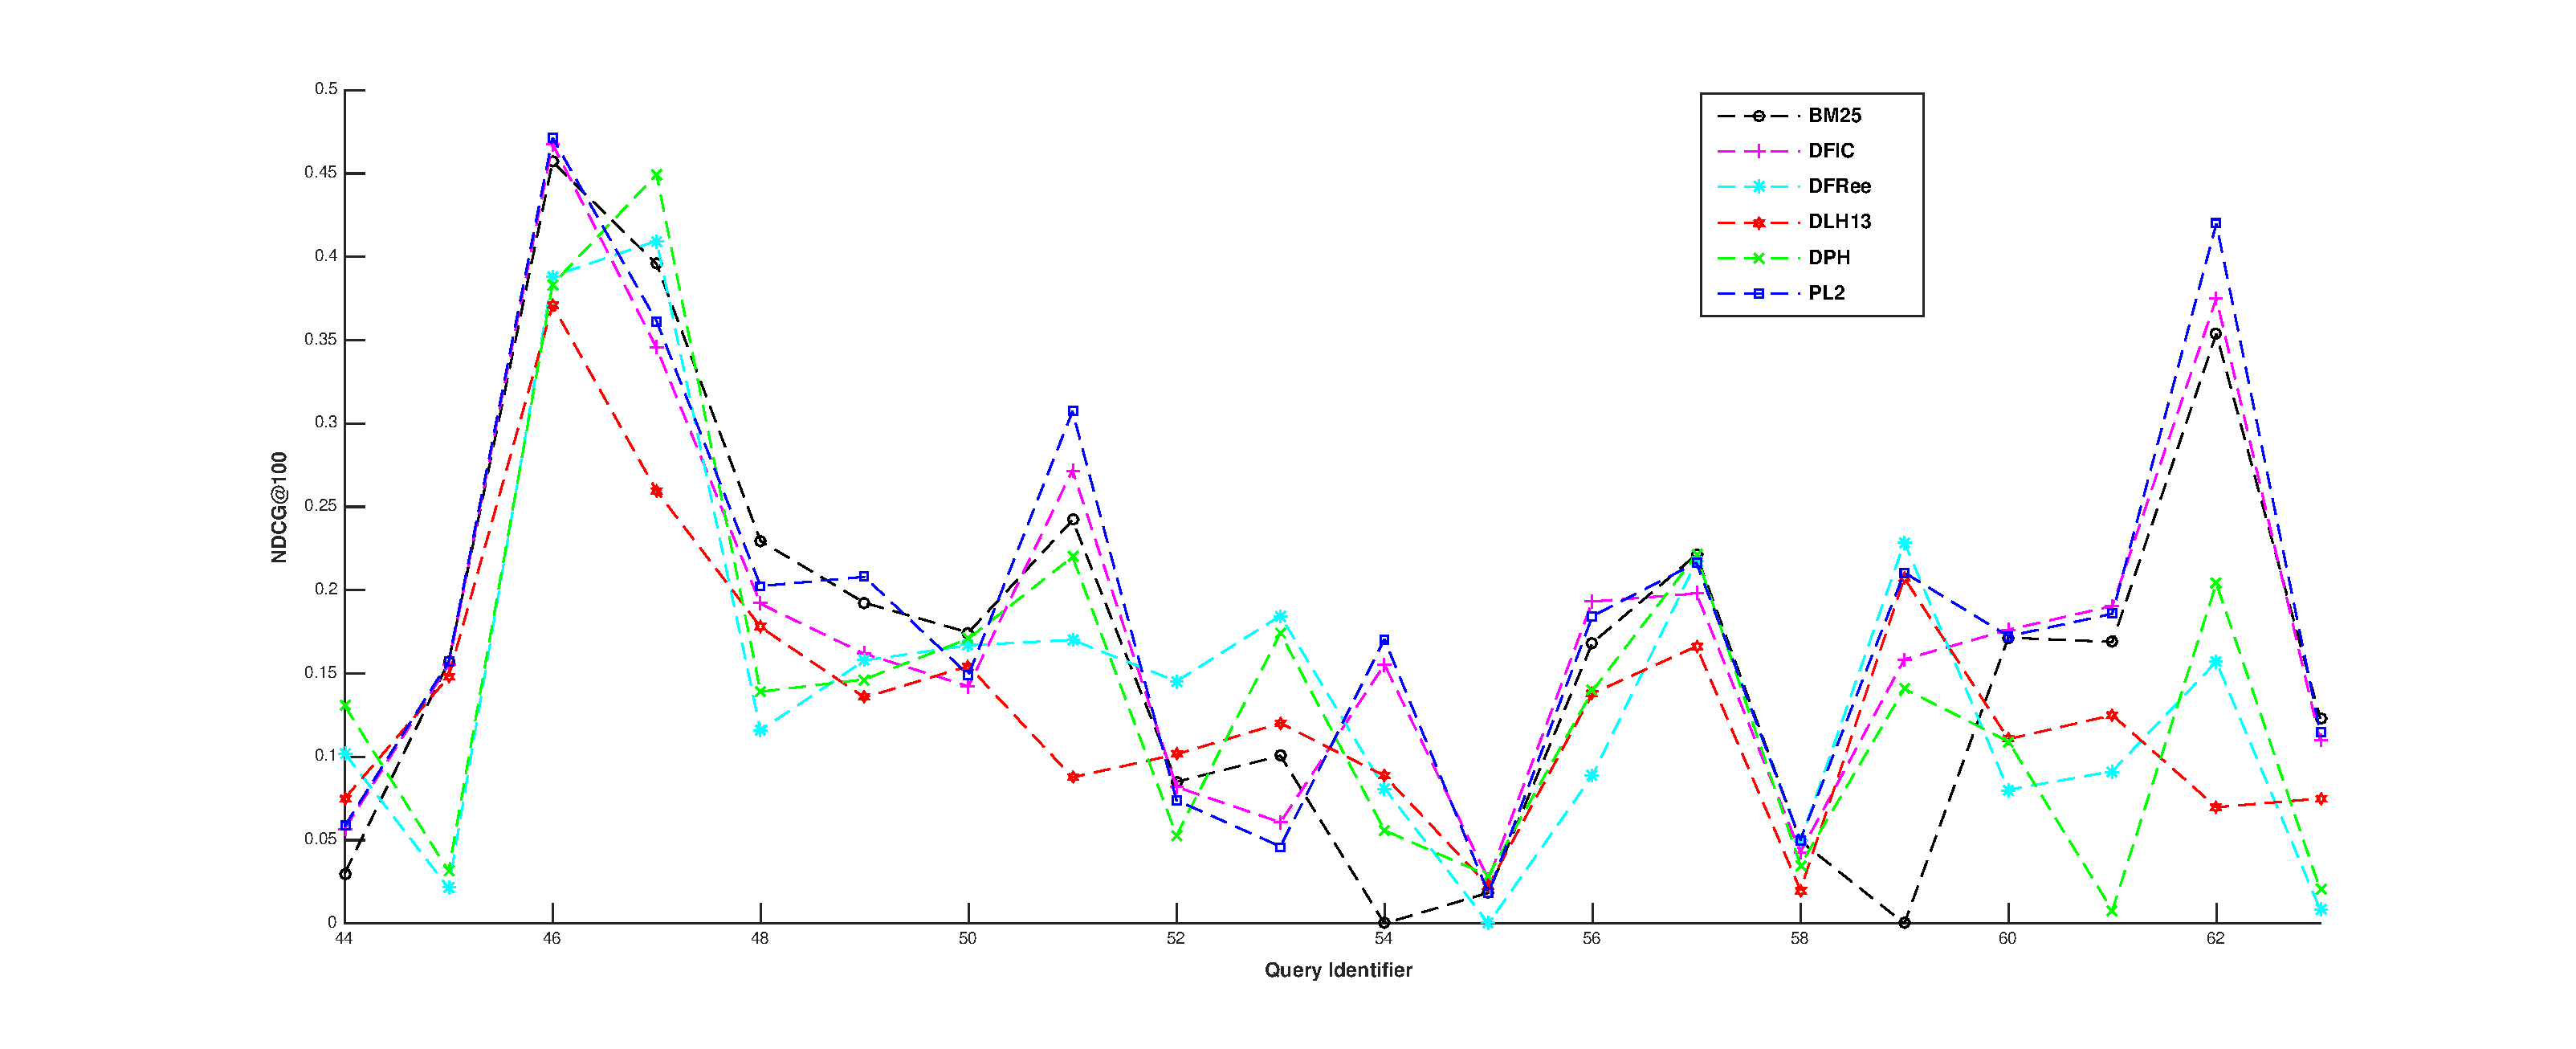
\includegraphics[width=\textwidth]{variance.eps}
\caption{The variance in effectiveness (NDCG@100) among eigtht models}
\label{fig1}
\end{figure}


\section{Research Questions and Hypotheses}
\label{1.3}

The statement of this dissertation is that the most effective term-weighting model can be accurately predicted from a number of candidate term-weighting models for each given query.
This is investigated in the context of a framework, called Selective Term Weighting (STW), where the success probability of a term-weighting model for a given query is estimated based on the queries it performed the best and the worst on the already seen test queries.
In the selective term weighting framework, the queries that the term-weighting model performed both the best and the worst are identified from the test query set.
The distance of a given test query to the identified query set is computed for each model and model with the highest probability is selected for the given query.

This dissertation analyze frequency distribution of terms on document collections in the context of IR.
This work develops a framework to selectively apply an appropriate term weighting model on a per query basis.
The prediction of a model among the candidate model set is based on the goodness of fit frequency distribution of query terms.
In particular, this dissertation addresses the following research questions:

\begin{enumerate}[label=\ac R\arabic*\kapa]
  \item For a given query, can the most effective term-weighting model be predicted among the current state-of-the-art models based on the frequency distributions of the queries' terms?
  \item Can a more effective or robust system be built by per-query application a model predicted among current state-of-the-art technologies than a system in which a single/individual model is uniformly applied to all queries? 
\end{enumerate}

\noindent Given these research questions, a number of hypotheses can be formally stated and tested.

\begin{enumerate}[label=\ac H\arabic*\kapa]
  \item For a given query, the most effective term-weighting model can be predicted with reasonable accuracy, by analyzing the frequency distributions of query terms on document collections.
  \item Different queries benefit differently from each term-weighting model and the retrieval effectiveness and robustness can be significantly enhanced if an appropriate term weighting model is used for each individual query. 
\end{enumerate}

\section{Contributions}

The main contributions of this dissertation are the introduction of the STW framework and the proposed use of chi-square goodness-of-fit test  
on frequency distributions of query terms for identifying similar queries.
In addition, this dissertation draws insights from a large set of experiments, involving three different standard corpora, two different search tasks, two different document representations and two different effectiveness measures calculated at various cutoff levels.
This illustrates the generalizability of the STW framework.

Furthermore, we thoroughly evaluate the accuracy, effectiveness and robustness of the STW framework on two different retrieval tracks, namely Web Track and Million Query Track.
In particular, a Web collection that contains over a half billion English documents and about one thousand queries are used in this evaluation.

This study makes some important contributions to the body of existing work in both selective IR and robust IR. 
This dissertation presents experiments of the selective term-weighting for robust retrieval based on frequency distributions of query terms. 
This is the first examination of the frequency distributions of query terms on document collections in text-based IR. 
This has not been done before. 
As a by-product, a new family of query features can be driven from the frequency distribution of query terms for to use in IR research area.

This work presents a unique evaluation methodology for selective retrieval approaches when there exist multiple candidates to choose from.
Three aspects of such evaluation: accuracy, effectiveness and robustness are considered at the same time.
Two natural baselines that any selective retrieval approach should outperform at the minimum are derived and described.

The present dissertation also reveals the organic connection between the selective IR and the robust IR that focused on avoiding significant failures caused by the poorly-performing queries. 
This connection has much to do with the true understanding/definition of a significant failure, and an appreciation of it helps to gain insight into the selective retrieval approach.

Indeed, significant failure is a vague concept. 
When does a retrieval system fail significantly? 
Can an effectiveness score of 0.2 or 0.6 be considered a failure for a particular query?
Whether a system performs poorly or not can only be meaningfully identified when it is \emph{relatively} compared to the \emph{other} systems.
For example, a system serves a query with the effectiveness measures of 0.6 and all the other systems attain effectiveness score greater than 0.7. 
Since the model in question is the least effective, we can call the score of 0.6 a significant failure.
On the other hand, a system can be the most effective with a score of 0.2 when the other systems return zero relevant documents.
Obviously effectiveness score of 0.2 is not a significant failure in this case.

These examples clearly demonstrate that significant failure must be defined in a relative manner.
There must be other systems to compare with. 
The magnitude of an effectiveness score alone is not enough to define it. 
This is where selective retrieval approaches come into play.
The interesting relationship between the selective retrieval approaches and the problem of robustness in retrieval effectiveness is that the selective approaches are natural solutions to the robustness problem.


\section{Outline of the Dissertation}
The remainder of this dissertation is organized as follows:

\paragraph{Chapter \ref{ch2}: Information Retrieval}
This chapter discusses relevant background material in IR. The main stages and models in IR are discussed, as well as the evaluation and the effectiveness measures in general. 
Term-weighting is shown to be a crucial aspect in IR.
Furthermore, the problem of robustness in IR effectiveness is explained.

\paragraph{Chapter \ref{ch3}: Related Work: Selective Information Retrieval}
This chapter describes the previous selective retrieval approaches proposed in the literature, as well as briefly surveys the existing studies on the query performance prediction.

\paragraph{Chapter \ref{ch4}: Our Approach: Selective Term Weighting}
This chapter describes the proposed selective term-weighting approach based on frequency distributions of query terms.

\paragraph{Chapter \ref{ch6}: Experimental Methodology}
This chapter provides the details of the experimental setup.

\paragraph{Chapter \ref{ch7}: Experimental Results and Analysis}
This chapter presents the experimental results and our interpretations of them.

\paragraph{Chapter \ref{ch9}: Concluding Remarks}
This chapter discuses concluding remarks and some interesting future directions for further research.

\bibliographystyle{elsarticle-harv}
\bibliography{References}
\end{document} 